\documentclass[twocolumn, 10pt, times, letterpaper]{article}
\usepackage[margin=1in]{geometry} %one inch margins
\usepackage{pslatex}
\usepackage{mathptmx}
\usepackage{listings}
\usepackage{achicago}
%\usepackage{fleqn} %sets equation to left
\usepackage{amsmath, amssymb}
%\usepackage{fancyhdr}
\usepackage{epsfig}
%\usepackage{pstricks,pst-node,pst-tree,pst-plot}
\usepackage{graphicx}
\usepackage{vmargin}
\usepackage{url}
\usepackage{tabularx}
%\usepackage{ccaption}


\usepackage{lastpage} % for the number of the last page in the document
\usepackage{fancyhdr}



% -------------------------------------------------------------------
% Different font in captions
% from http://dcwww.camp.dtu.dk/~schiotz/comp/LatexTips/LatexTips.html
\newcommand{\captionfonts}{\it}
\makeatletter  % Allow the use of @ in command names
\long\def\@makecaption#1#2{%
  \vskip\abovecaptionskip
  \sbox\@tempboxa{{\captionfonts #1: #2}}%
  \ifdim \wd\@tempboxa >\hsize
    {\captionfonts #1: #2\par}
  \else
    \hbox to\hsize{\hfil\box\@tempboxa\hfil}%
  \fi
  \vskip\belowcaptionskip}
\makeatother   % Cancel the effect of \makeatletter
% -------------------------------------------------------------------

% PDF Links --------------------------------------------------------
%% \usepackage[ps2pdf,colorlinks]{hyperref}
%%  \hypersetup{backref, %
%%    colorlinks=true, %
%%    linkcolor=black, %
%%    anchorcolor=black, %
%%    citecolor=black, %
%%    filecolor=black, % Color for URLs which open local files.
%%    menucolor=black, % Color for Acrobat menu items.
%%    pagecolor=black, % Color for links to other pages.
%%    urlcolor=black, %
%%    pdftitle={}, %
%%    pdfauthor={}, %
%%    pdfsubject={}, %
%%    pdfkeywords={}%
%%  }
% Fuzz -------------------------------------------------------------------
\hfuzz4pt % Don't bother to report over-full boxes if over-edge is < 2pt
\vfuzz=\hfuzz
% THEOREM Environments ---------------------------------------------------
\newtheorem{definition}{Definition}
\newtheorem{assumption}{Assumption}
\newtheorem{theorem}{Theorem}
\newtheorem{lemma}{Lemma}
\newtheorem{corollary}{Corollary}
\newtheorem{proposition}{Proposition}
\newtheorem{algorithm}[theorem]{Algorithm}
\newcommand{\rbox}{ \qed }

\renewcommand{\Re}{{\mathbb R}}
\newcommand{\Na}{{\mathbb N}}
\newcommand{\Z}{{\mathbb Z}}

% Depth of table of contents -----------------------------------------
\setcounter{tocdepth}{2}

%QED box, from the TeXbook, p. 106. ----------------------------------
\newcommand\qed{{\unskip\nobreak\hfil\penalty50\hskip2em\vadjust{}
    \nobreak\hfil$\Box$\parfillskip=0pt\finalhyphendemerits=0\par}}


% Line spacing -----------------------------------------------------------
\newlength{\defbaselineskip}
\setlength{\defbaselineskip}{\baselineskip}
\newcommand{\setlinespacing}[1]%
           {\setlength{\baselineskip}{#1 \defbaselineskip}}
\newcommand{\doublespacing}{\setlength{\baselineskip}
                           {2.0 \defbaselineskip}}
\newcommand{\singlespacing}{\setlength{\baselineskip}{\defbaselineskip}}
\newcommand{\onehalfspacing}{\setlength{\baselineskip}
                           {1.5 \defbaselineskip}}

\hyphenation{TRNSYS}

% Page layout ------------------------------------------------------------
% see LaTeX Companion, p. 83ff
\setlength{\hoffset}{-37 mm}
\setlength{\topmargin}{0mm}%
\setlength{\textwidth}{16.8cm}
\setlength{\textheight}{22.7cm}
\setlength{\headheight}{31.75mm}
\setlength{\headsep}{12pt}
%\setlength{\footheight}{12pt}
\setlength{\footskip}{12pt}
\setlength{\parindent}{0pt}

%\setlength{\columnsep}{8mm}
\setlength{\columnsep}{0.25in}
\setcounter{secnumdepth}{-2} % to avoid numbering
%\setlength{\mathindent}{0mm}

% -------------------------------------------------------------------------
% Section headings
% p. 27
 \makeatletter
 \renewcommand{\section}{\@startsection
   {section}%            %the name
   {0}%                  %the level
   {0mm}%                %the indent
   {6pt}%               %the beforeskip
   {3pt}%                %the afterskip
   {\noindent \fontsize{12}{14}\selectfont \underline}}  %the style
%   {\noindent \large \sc \underline}}  %the style

 \renewcommand{\subsection}{\@startsection
   {subsection}%            %the name
   {1}%                  %the level
   {0mm}%              t  %the indent
   {6pt}%               %the beforeskip
   {3pt}%                %the afterskip
  {\noindent \fontsize{10}{12}\selectfont \bf}}  %the style
%   {\noindent \bf}}  %the style
 \makeatother

% Make capitalized reference header for IBPSA
\renewcommand{\refname}{REFERENCES}

\newcommand{\authorfont}{\fontsize{12}{14}\selectfont}
\newcommand{\titlefont}{\fontsize{12}{14}\selectfont \bf}
% -------------------------------------------------------------------------
\pagestyle{empty}

% -------------------------------------------------------------------------
% Contents ----------------------------------------------------------------
\begin{document}
\fancypagestyle{empty}{%
  \fancyhf{}% Clear header/footer
  \renewcommand{\headrulewidth}{1.5pt}
  \fancyhead[L]{\includegraphics [width=1.5in] {images/logo_new.jpg}}
% conference logo
  \fancyhead[R]{2018 Building Performance Modeling Conference and \\ SimBuild co-organized by ASHRAE and IBPSA-USA \\ Chicago, IL \\ September 26-28, 2018}% header text
}

%\onehalfspacing
\bibliographystyle{achicago}
\renewcommand{\SCduplicate}[1]{#1}
\date{}
\title{\vspace{-9mm} \titlefont %
PAPER PREPARATION GUIDE AND SUBMISSION INSTRUCTIONS
FOR 2018 BUILDING PERFORMANCE MODELING CONFERENCE and SIMBUILD CO-ORGANIZED BY ASHRAE AND IBPSA-USA}
\author{%
\authorfont{John Modeller$^1$, Jane Simulator$^2$, and Another Author$^3$}\\
\authorfont{$^1$Technical University, Cambridge, MA}\\
\authorfont{$^2$Another Institution, Some City, Some Country}\\
\authorfont{The names and affiliations SHOULD NOT be included in the draft submitted for review.}\\
\authorfont{The header consists of 10 lines with exactly 14 point spacing.}\\
\authorfont{The line numbers are for information only. The last line below should be left blank.}\\
\authorfont{~}\\ % used to add blank lines
\vspace{-14mm}
}
\maketitle
\thispagestyle{empty}

% --------------------------------------------------------
\section{ABSTRACT}

We develop an integrated solution for incorporating ``digital twins” of real buildings into existing SCADA systems, which enables real-time prediction and advanced control. 
These digital twins are either EnergyPlus (E+) or data-driven (D+) building models, whose input and output variables are mapped to analogous real building OPC tags and track the real-time operation of the building.
An E+ digital twin can be used to provide predictions of the building’s performance in different weather, usage, and energy pricing scenarios, which allows for accurate assessment of different control strategies. 
However, it is not suitable for optimization and predictive control due to its complexity. 
We develop scalable D+ digital twin based on Gaussian Processes (GP) for accurate prediction and advanced control. 
A D+ digital twin is much easier, faster, and less expensive to train than developing and tuning an E+ model, while still providing accurate power forecasts and being suitable for control. 
Data-driven Model Predictive Control (MPC) optimizes control inputs of the predictive D+ model for energy curtailment with thermal comfort guarantees in demand response applications.
The MPC controller is integrated into the SCADA environment, demonstrating real-time in-the-loop control of D+ digital twins.

%%% Local Variables:
%%% mode: latex
%%% TeX-master: "main"
%%% End:


% --------------------------------------------------------
\section{INTRODUCTION}
\label{S:intro}

Efficient control of buildings requires high fidelity models that capture the evolution of the state of the building with time, for example, how the power consumption and zone temperature are affected when the chilled water or the supply air set points are changed with time or when outside weather conditions are different.
Model Predictive Control (MPC) uses such models to predict the state of the building over a finite horizon and optimize the performance with a given objective like load curtailment while meeting thermal comfort and operation constraints.

To this end, the classes of models that are most widely studied in the literature use first principles based on physics. 
These include the \textit{white box} models typically based on high fidelity simulation software like EnergyPlus (E+) \cite{Deru2011} and TRNSYS \cite{Transys1975}, and the \textit{grey box} models based on Resistor Capacitance (RC) networks \cite{Deng2010}.
The user expertise, time, and associated sensor costs required to develop such models of a single building are very high.
This is because such models require detailed information about the geometry of a building, design and equipment layout plans, material properties, and equipment and operational schedules. 
%There is always a gap between the modeled and the real building and the domain expert must then manually tune the model to match the measured data from the building.
Moreover, the modeling process also varies from building to building with the construction and types of installed equipment. 
%Another major downside with physics-based modeling is that enough data is not easily available and guesses for parameter values have to be made, which also requires expert know how.
After several years of work on using first principles based models for peak power reduction, and energy optimization for buildings, multiple authors \cite{Sturzenegger2016,vzavcekova2014} have concluded that the biggest hurdle to mass adoption of intelligent building control is the cost and effort required to capture accurate dynamical models of the buildings.

We take an alternative route to the physics-based approach, i.e.~\textit{black box} modeling based on machine learning algorithms to learn a digital twin of the underlying physical system, a building in this case.
Our approach reduces the cost and time to model the buildings by an order of magnitude \cite{JainICCPS2018,JainCDC2017,JainACC2017,nghiemetal16gp,behletal15dradvisor}.
We learn data-driven (D+) models using only historical data available via sensors already installed in the buildings -- thermostats, multimeters -- and historical weather data.
The D+ models can not only be used for prediction but also for real-time MPC.
These models are scalable and integrate seamlessly to the existing Supervisory Control and Data Acquisition (SCADA) software or the Building Energy Management Systems (BEMS).

Although expensive to build, the E+ models are useful to simulate the behavior of the building. For example, building operators use E+ as an isolated testbed to analyze different control strategies and receive immediate feedback without having to implement the strategies on the real building.
The drawback of E+ models is that they cannot be used for MPC.
On the other hand, as we will show, the D+ models are much less expensive to build and they can be used for simulating the response of the real building as well as for real-time MPC.

\todo[inline]{what is wrong with current SCADA?}
\begin{figure}
	\missingfigure[figwidth=\linewidth]{problem setup}
	\caption{Problem setup}
	\label{F:intro}
\end{figure}

In this paper, we present an end-to-end architecture for modeling and HVAC control of large scale buildings efficiently using machine learning, see Figure \ref{F:intro}. 
We explain and demonstrate with examples our complete pipeline starting from tools for data acquisition from existing SCADA/BEMS to learning accurate control-oriented data-driven models using Gaussian Processes (GP) to real-time predictive control with high confidence.

% --------------------------------------------------------
\section{DATA ACQUISITION \& COMMUNICATION}

In a building automation system, a Supervisory Control and Data Acquisition (SCADA) system is commonly used by the operators to manage individual buildings or a campus of buildings. 
It interfaces directly with building sensors and controllers through open source protocols like BACNet or OPC. 
SCADA software also provides a dashboard interface for operators to view live or historical data feeds from sensors and an easy way for operators to change control setpoints remotely. 
Additionally, it may also offer a Historian database to store historical data values for future reference or data analysis.
See Figure \ref{F:intro} for an illustration of a typical SCADA system.

There are two main limiting factors in bridging digital twins with existing SCADA software.
First, most SCADA software are self-contained and the features are limited to those provided by the vendor.
Building operators cannot view the results from E+/D+ models on the same SCADA software used for real-time monitoring because it is not clear how we can communicate between the E+/D+ models and existing SCADA software to acquire the data tags required by E+/D+ models for simulation and control, and to show the generated results on the dashboards.
Second, if the digital twin is an E+ model, we need an external library like MLE+ \cite{bernaletal12mti} to design a controller in a scripting language such as MATLAB.
This is because EnergyPlus only allows manually coded rule-based control strategies.
Since Python is a popular programming language for data science and machine learning, we need an alternative to MLE+ for Python. 

In this work, we use the open interface OPC to connect EnergyPlus with any existing SCADA software that supports OPC for real-time data communication. 
We call this the EnergyPlus-OPC bridge.
By representing inputs to and outputs from EnergyPlus as OPC tag structures, we make the integration into existing SCADA software significantly easier since the simulated building will appear as a real building to the SCADA software.
Furthermore, since our machine learning models are written in Python, we develop a library to interface Python and EnergyPlus called \texttt{pyEp}, an equivalent to MLE+ for Python.
We show how this library allows for intelligent control of buildings using D+ models and testing on E+ models.
The transition from testing on E+ models to testing on real buildings can be made seamlessly through the SCADA system.

% In summary, E+ models cannot be used for designing advanced controllers like MPC. 
% But an interface like MLE+ (MATLAB) and \texttt{pyEp} (Python) allows the users to test manual control strategies more conveniently.
% On the other hand, as we show in Section \ref{S:dpc}, D+ models, are suitable for MPC.
% In the examples that will follow, we will test a controller based on a D+ model on an E+ model as a plant (substitute for a real building).
% This setup is shown in Figure \ref{F:control}.
% The EnergyPlus-OPC bridge allows us to interface the E+/D+ models to the SCADA software and enables to study a closed-loop response of this building.
% Once the optimal setpoints are obtained from MPC, and the corresponding digital twin response behavior can be viewed in real time in a commercial SCADA dashboard.

The case studies presented later in this paper use the setup shown in Figure \ref{F:control}, in which a data-driven controller based on a D+ model acts on an E+ model as a plant.
The EnergyPlus-OPC bridge allows us to interface an E+/D+ model to the OPC server and thus to the SCADA software for real-time monitoring and closed-loop control of the building.
The setpoints obtained from the controller and the corresponding responses from the digital twin can be viewed in real time in a commercial SCADA dashboard.

\begin{figure}[t]
	\centering
	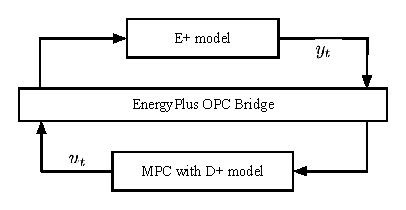
\includegraphics[width=0.4\textwidth]{images/control.eps}
	\caption{The MPC controller runs in Python using the D+ models and applies the optimal inputs to the E+ model. The communication is made possible using the \texttt{pyEp} library and the OPC connection.}
	\label{F:control}
\end{figure}

\subsubsection{EnergyPlus-OPC Bridge}

Our EnergyPlus-OPC bridge provides the EnergyPlus input and output variables as OPC tags to be read by any OPC client.
The user is able to configure the simulation for any number or type of buildings and can run each individually on different schedules.
To see the simulation in progress, the operators only need to view the tag using an OPC client, as they would for any other data source.
By writing to one of the input tags, the operators can change the input setpoints to EnergyPlus and see the response of the building.
For more advanced control of the building, operators can use our MPC controller based on D+ models.
The service supports the running of multiple EnergyPlus instances, creating a campus of isolated buildings.
The buildings are simulated synchronously, so that their simulations are always kept at the same time. % sequentially, but kept at the same time, so that the first building only advances a time step when all other buildings are at the same time.
This capability can be useful when looking at aggregate power consumption and synthesizing control strategies involving multiple-building curtailment.
For communication between EnergyPlus and Python we use \texttt{pyEp}.

\subsection{pyEp: A Python EnergyPlus Interface}

Currently, EnergyPlus supports external programs through the Building Controls Virtual Testbed (BCVTB), built on top of Ptolemy II, and the Functional Mockup Interface (FMI) standard. 
Using BCVTB, the users can couple and define data flows between various modeling and simulation programs, such as TRNSYS or Simulink. 
These simulation environments, while comprehensive, are still constrained by the capabilities of the software. 
MLE+ provides a solution to this problem, allowing the end-users to directly control the progress of an EnergyPlus simulation by writing MATLAB code. 
In recent years, Python has become a popular language for data science and machine learning, in academia and especially in industry. % but   with many advanced open-source libraries like TensorFlow \cite{Abadid} and Scikit-learn \cite{Pedregosa2011} being used widely in industry and academia.
The \texttt{pyEp} library connects the myriad of Python libraries with existing technologies in the building modeling and simulation communities.
For example, in our case studies depicted in Figure \ref{F:control}, we obtain data from EnergyPlus to learn D+ models, which are used for synthesizing building control strategies, then evaluate these strategies in closed-loop simulation with EnergyPlus.
These steps are made possible by \texttt{pyEp}.
%This communication has been made possible with the \texttt{pyEp} library.

The \texttt{pyEp} library is designed to be lightweight and flexible. 
The core class is \texttt{ep\_process}, which provides simple read and write capabilities with EnergyPlus. 
Each \texttt{ep\_process} instance corresponds to one EnergyPlus building, and is independent of all other \texttt{ep\_process} instances. 
% This means that \(\mathtt{idf}\) files (format specific to EnergyPlus) built for different EnergyPlus versions, or buildings with different weather files, can be run together in a campus-like co-simulation.
This allows for multiple EnergyPlus models being run together in a campus-like co-simulation. 
An example using the Department of Energy (DoE) provided LargeOffice building model is included in the installation. 
For an EnergyPlus IDF model file to be used with \texttt{pyEp}, it must have the \texttt{ExternalInterface} configured, as well as an associated \texttt{variables.cfg}, specifying the inputs and outputs to the \texttt{ExternalInterface}.
\texttt{pyEp} is available on the Python Package Index (PyPI) and can be installed with the command \verb|pip install pyEp|.
Its documentation can be found at \url{https://pypi.org/project/pyEp/}.

\subsubsection{System Architecture}

\begin{figure}[t]
	\centering
	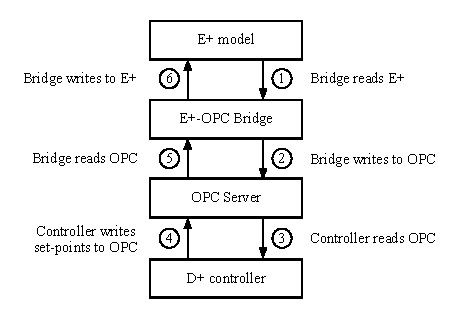
\includegraphics[width=0.5\textwidth]{images/architecture.eps}
	\caption{Communication sequence for data exchange.}
	\label{F:architecture}
\end{figure}


The EnergyPlus-OPC bridge requires two processes to start and control a simulation over OPC. 
The first is the bridge itself, which can be started once and left in the background indefinitely. 
The second is a controller, which determines which setpoints to write to the bridge at what time during the simulation. 
The role of the bridge is to handle communication between EnergyPlus and the OPC server. 
The role of the controller is to control the inputs at every time step of the EnergyPlus co-simulation by writing to the OPC server.
The communication sequence for data exchange is shown in Figure \ref{F:architecture}.
%At time step $t$, the bridge first writes the outputs from EnergyPlus at the previous time step $t-1$. 
%The controller then reads the outputs and uses them to determine the next set of inputs to write to the EnergyPlus input tags. 
%For a controller running on a fixed schedule, it would use the simulation time to determine what setpoints to write. 
%A more energy-savings focused controller might use the current power consumption to determine if a curtailment strategy should be implemented instead. 
%After the controller writes them to the input OPC tags, the bridge reads them and passes them into EnergyPlus. 
The same process follows for the next building, until all have been incremented forward by one time step.
The communication protocol ensures that every input and output are read to the correct EnergyPlus building, and that delays in the network communications do not cause the controller and bridge to become out-of-sync with each other. 
The exchange of information is not real-time dependent, so human operators can change the inputs time step by time step at any pace. 
The controller can also preemptively stop a simulation by terminating the controller process. 
Changes to a prescribed schedule can also be made, and the simulation restarted again without needing to restart the bridge process. 
This allows for faster and easier changes with less time overhead between simulation runs.
Specific syntax can be found in the documentation. 
The bridge should only be restarted if different EnergyPlus buildings need to be used.

This bridge-controller design provides great flexibility in how the user can make use of EnergyPlus. 
Users can freely modify the controller to customize the simulation parameters. 
A simple schedule based controller can be made with basic knowledge of Python. 
Alternatively, more complex model-based controllers like MPC as in Section \ref{S:dpc} can also be implemented and evaluated.
Two example controllers are included in the \texttt{pyEp} library. 
The first controller implements a setpoint schedule in Python and shows how to read/write from the controller to EnergyPlus. 
The second controller implements a setpoint schedule based on a formatted csv file. 
% No knowledge of Python is needed to edit and run a custom setpoint schedule.

\subsubsection{Requirements}

The provided controllers use the OpenOPC library to connect to an OPC server, but other methodologies may be used if the communications paradigm is followed. See \texttt{pyEp} documentation for more details.
Additionally, the free Matrikon OPC Server Simulator is used as the default server.
Included with \texttt{pyEp} is a server configuration XML generator that automatically creates the correct OPC Tree Tag structure for the Matrikon Server. 
The \texttt{pyEp} core module, linking EnergyPlus to Python, is supported for Python 2.7 and 3.x, while the EnergyPlus-OPC bridge requires Python 2.7.

%%% Local Variables:
%%% mode: latex
%%% TeX-master: "main"
%%% End:


% --------------------------------------------------------
\section{SUBMISSION INSTRUCTIONS}
\begin{enumerate}
\item
{\it In light of the double-blind review, please do not include your name and affiliation on the draft submitted for review.}
\item
Please convert your document to PDF format. Other formats are NOT acceptable.
\item
The filename must reference your ID\#. 
\item
Please submit your paper through Conftool. Your specific link was included in your abstract acceptance letter (.  If your paper does not meet the submission requirements, your file will not be processed for review. 
\item 
You will receive a confirmation via e-mail if your paper is successfully uploaded. (BPACS 2018 -- Abstract decision email) You may submit your Conference Paper in advance of the February 2 deadline. You will be notified of the results of the peer review in March and may be asked to submit revisions for re-review.
\end{enumerate}


% --------------------------------------------------------
\section{CONCLUSION}

This paper presented a set of methods and tools to incorporate ``digital twins'' of real buildings into existing SCADA systems.
We proposed a data-driven modeling approach using Gaussian Process to quickly and inexpensively capture a model of a building solely from its measurement data.
This type of models, called D+ models, together with EnergyPlus (E+) models of buildings serve as ``digital twins'' of the buildings.
In addition to requiring significantly lower cost and effort to develop, compared to E+ models, D+ models are more suitable for Model Predictive Control (MPC) and more adaptive to changes in the buildings.
Two applications of MPC with D+ models were formulated for demand-tracking control and climate control with minimum energy.

We developed an EnergyPlus-Python bridge, called pyEp, to interface Python code with EnergyPlus to perform co-simulations, which is useful for implementing advanced algorithms such as machine-learning-based modeling and optimization-based control.
We also developed an EnergyPlus-OPC bridge, which completes our toolchain for integrating E+ and D+ models into SCADA systems.
Through OPC tag mappings, these digital twins can directly exchange data with a SCADA system, receiving control commands and returning measurement values as if they were real buildings.
For the first time, our toolchain has enabled seamless real-time in-the-loop prediction and advanced control of both software buildings and physical buildings within the same SCADA environment.
The toolchain was demonstrated in a case study, which showed the effectiveness of both our software and our proposed data-driven MPC approach for buildings.

\todo[inline]{Well, any idea whether and how we want to extend this work?}

%%% Local Variables:
%%% mode: latex
%%% TeX-master: "main"
%%% End:



\bibliography{references}

% --------------------------------------------------------
\section{NOMENCLATURE}

\begin{tabular}{p{12mm}p{55mm}}
  $e$        & error \\
  $E$        & energy \\
  $T$        & temperature \\
\end{tabular}

 

\end{document}